%%%%%%
%%%%%% Chapter 2
%%%%%%

\chapter{Stochastic Variables}
Since the notion of random variables will be essential
for the understanding of stochastic methods this chapter will be 
devoted to the introduction of the fundamental concepts of 
probability theory.

%%%%%%%%%%%%%%%%%%%%%%%%%%%%%%%%%%%%%%%%%%%%%%%%%%%%%%%%%%%%%%%%%%
\section{The nature of probabilities}
In the previous chapter we have already made use of probabilistic 
notions in an intuitive way. However, we have not asked the 
following question: What are probabilities? How can we formulate 
the notion of probability in such a way that it is useful for 
physical applications?

Essentially, there are three possible definitions of probability
\cite{BRODY}:
a) the axiomatic interpretation, b) the frequency interpretation, and
c) the ensemble interpretation.


\subsection{The axiomatic interpretation}
The axiomatic definition \cite{FELLER} of probabilities has been proposed by 
Kolmogorov in 1933. The formal objects to which we want to 
attribute probabilities are called {\em events} and are subsets
of a basic set $\Omega$ which is called the {\em event space} or in 
physical applications the {\em phase space}. If the event $e$ 
belongs to $\Omega$, so does its complement $\Omega - e$ also; the 
null event $\oslash$ is therefore also in $\Omega$. Events 
containing only one member of $\Omega$ are called the elementary events
of $\Omega$.

A function $P(e)$, called the {\em probability} of $e$ can be 
assigned to each event $e$ in $\Omega$. The function $P(e)$ has
the following properties:

(i) $P(e) \ge 0$ for all $e$ in $\Omega$;

(ii) $P(\Omega) = 1$;

(iii) If $e_1, e_2, \ldots $ are in $\Omega$ and are pairwise
disjoint, i.e., $e_i \cap e_j = \oslash$ when $i \ne j$, then
$P(e_1 \cup e_2 \cup \ldots ) = P(e_1)+P(e_2) + \ldots$.

It follows immediately from the above three axioms that

(iv) If $\bar{e}$ is the complement of $e$, i.e., the set of all 
events which are not in $e$, then
$P(\bar{e}) = 1- P(e)$;

(v) $P(\oslash) = 0$.



\subsection{The relative frequency interpretation}
In his attempt to axiomatize probability theory, von Mises
introduced in 1919 the notion of a {\em Kollektiv}, which stands
for a single infinite sequence of random events such as the 
outcomes of throwing a coin. He defined then the probability of some 
event to be the limit of its relative frequency in such a series of 
observations when the series becomes infinitely long (the 
Kollektiv) \cite{COMPAGNER,BRODY}. 
If we denote by $n$ the number of data in the series,
by $m(e)$ the number of times the event is observed in it, then
the probability $P(e)$ is defined as
\begin{equation}
P(e) = \lim_{n \rightarrow \infty} \frac{m(e)}{n}.
\end{equation}
Of course, such a series of events must have the property that any 
infinite subsequence in it must have the same limit. 

The problem with this definition is the following one: How can any 
sequence of experimental data, which will be always be finite, 
have the properties of such a Kollektiv? In practice the 
relative frequencies for subsequencies will always differ from 
that in the main sequence.

To illustrate the problems with the frequency interpretation of
probabilities we consider the following example. We throw a die 
$n$ times and
look at the relative frequency $m(4)$ of the outcome of throwing a 
4. This experiment will be simulated with the help of the 
following program.

{\bf Listing of the program relfreq.}
\inputlisting{./Listings/relfreq.m}

The result of an experiment for up to 400 throws is shown in Fig. 
(\ref{F_FRELFREQ}). Running the program again we observe 
another approach to the asymptotic
value. We recognize immediately the difficulties with von Mises 
definition of probability.
\begin{figure}
\label{F_FRELFREQ}
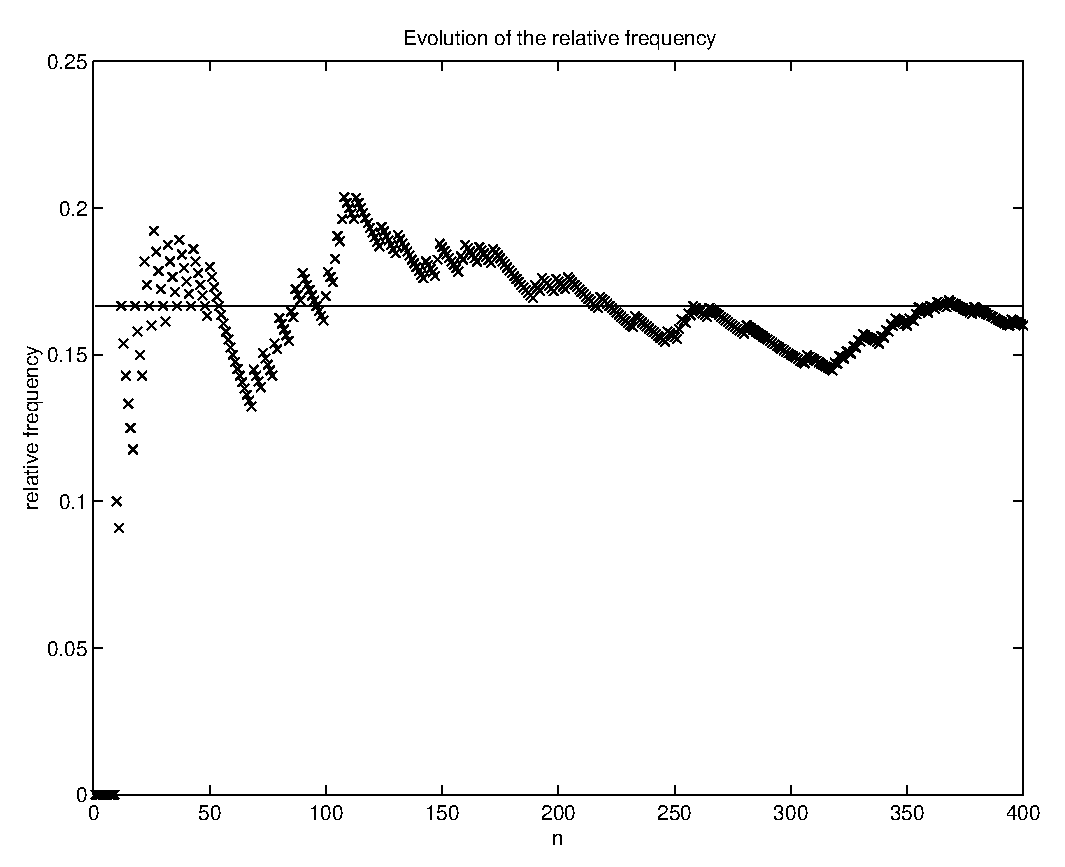
\includegraphics[width=10cm]{frelfreq.eps}
\caption{Simulation of the evolution of the relative frequency of throwing
a 4 in play of die.}
\end{figure}

\subsection{The ensemble interpretation}
We know from statistical mechanics  the notion of {\em ensemble}. An
ensemble is a collection of a large number $N$ of equally prepared
systems (equal models). A simple example is the microcanonical
ensemble, 
which is the
ensemble of all microstates in phase space, which are characterized by
fixing the macroscopic values for the the energy $E$, the volume $V$
and the number of particles $N$.

The abstract concept of an ensemble allows naturally the definition
of a mean value. We have to consider two cases:

(i) The ensemble contains a finite, discrete number of models: 
Let $n$ be the number of models and $Q(i)$ the interesting quantity in
model $i$. The ensemble mean value $\langle Q \rangle$ is then defined
as
\begin{equation}
\langle Q \rangle = \sum_{i=1}^n \frac{Q(i)}{n}.
\end{equation}

(ii) The models are characterized by some continuous parameter, i.e.,
the initial positions of molecules in a gas: If we name the continuous
parameter $\omega$, the phase space as $\Omega$ , and $n(w)$ a weight
function characterizing the ensemble, then
\begin{equation}
\langle Q \rangle = \frac{ \int_{\Omega} Q(\omega) dn(\omega)}
                         {\int_{\Omega} dn(\omega)}.
\end{equation}
Usually, the function $n(\omega)$ can be derived on the basis of the
theoretical model on which the ensemble relies upon. 

Let us consider as a simple example from equilibrium statistical 
mechanics a gas consisting of $N$ particles. The microstates of 
the system are the points $(q,p) = (\vec{r}_1, \vec{r}_2, \ldots, \vec{r}_N,
\vec{p}_1,\ldots, \vec{p}_N)$ in the 6--dimensional phase space.
The probability to find the microsystem at time $t_0$ in a volume 
element $dV=d^{3N}qd^{3N}p$ around $(q,p)$ is given by
\begin{equation}
dw(q,p) = \rho(q,p) d^{3N}qd^{3N}p,
\end{equation}
where $\rho(q,p)$ is the distribution function. For the 
microcanonical ensemble  the distribution function $\rho$ simply 
reads
\begin{equation}
\rho(q,p) = \left\{ 
\begin{array}{ll}
c= {\rm const}, &{\rm for} \quad E-\Delta \le H(q,p) \le E, \\
0, &{\rm otherwise}
\end{array} \right.
\end{equation}

Probabilities can be introduced as a special kind of ensemble 
average. Let $A$ be a property, which 
the members of the ensemble may have or not and let us define an indicator
function
\begin{equation}
\chi_A(\omega) = \left\{ 
\begin{array}{ll}
1, & {\rm if \quad member \quad labelled} \quad \omega {\rm \quad has 
\quad property\quad} A \\
0, & {rm if not}.
\end{array}\right.
\end{equation}
The probability of $A$ in the ensemble is  simply defined as 
the ensemble average of $\chi_A(\omega)$
\begin{equation}
P(A) = \langle \chi_A(\omega) \rangle = 
\frac{\int_{\Omega} \chi_A(\omega) dn(\omega)}{\int_{\Omega} 
dn(\omega)}.
\end{equation}
The probability is the relative weight in the ensemble of those 
members that have the property $A$. In the case of a discrete 
ensemble the above definition of probability reduces to a sum over
the members of the ensemble having the property $A$
\begin{equation}
P(A) = \sum_{i=1}^{n} \frac{\chi(i)}{n},
\end{equation}
i.e., the probability is the relative frequency of the members 
having the property $A$ in the ensemble.

It is clear that from the above definition of probability its is
possible to derive the Kolmogorov axioms of probability theory.

It is important to stress that the
ensemble is a purely theoretical construction and has to be adapted 
to the physical situation of interest as we will see in the future chapters. 
Furthermore, it is to be noted that the ensemble 
interpretation  allows the definition of time dependent 
probabilities,
i.e.,
\begin{equation}
P(A,t) = \langle \chi_A(t) \rangle,
\end{equation}
which are of fundamental importance while studying stochastic 
processes.

%%%%%%%%%%%%%%%%%%%%%%%%%%%%%%%%%%%%%%%%%%%%%%%%%%%%%%%%%%%%%%%%%%
\section{The definition of stochastic variables}
A stochastic variable $X$ is an object which is defined by a space 
of states (space of events, phase space) and by a probability 
density over this set. The space of state may be discrete, e.g. 
the numbers 1,2,3,4,5,6 for a play of dice or the number of 
molecules in a chemical reaction, as well as continuous, e.g.
the velocity of a Brownian particle. Of course, the space of state
may also be discrete and continuous at the same time, e.g., the
energy of an electron in the presence of some binding centers.
When sampling a one dimensional continuous stochastic variable $X$,
the probability to find some value in the infinitesimal interval
$(x,x+dx)$ will be expressed symbolically by
\begin{equation}\label{DENSITYDEF}
P(x) dx \equiv {\rm Prob} \{X\in [x,x+dx] \},
\end{equation}
which defines the probability density $P(x)$ associated with the 
stochastic variable $X$. It follows immediately from the above 
equation and from the addition law of
probability theory that the probability to sample a value of $X$
in the interval $[a,b]$ is given by
\begin{equation}\label{DENSITYDEF2}
\int_a^b dx P(x) = {\rm Prob}\{ X \in[a,b] \}.
\end{equation}
It is evident from Eqs. (\ref{DENSITYDEF}) and (\ref{DENSITYDEF2}) that 
the probaility density is non--negative, i.e. $P(x) \ge 0$ and 
that it is normalized
\begin{equation}
\int_{-\infty}^{\infty} dx P(x) = 1.
\end{equation}
For later convenience we remark that the probability density may 
contain also sums over $\delta$--functions. For example $P(x)$ can 
also have the form 
\begin{equation}
P(x) = \sum_n p_n \delta(x-x_n) + \tilde{P}(x),
\end{equation}
where
$\tilde{P}(x) \ge 0$, $p_n \ge 0$, $\tilde{P}$ integrable  
and the normalization condition is
\begin{equation}
\sum_n p_n + \int dx \tilde{P}(x) =1.
\end{equation}

The distribution function $F$ of the stochastic variable $X$ is 
defined by 
\begin{equation}
F(x) \equiv {\rm Prob}\{X \le x\}.
\end{equation}
The density function and the distribution function are related by 
the equation
\begin{equation}
F(x) = \int_{-\infty}^x dx' P(x'),
\end{equation}
or equivalently by $F'(x)= P(x)$.

\subsection{Further characterization of stochastic variables}
A stochastic variable is completely defined by the space of states 
and by the probability density function. However, it is helpful to 
introduce some other quantities in order to characterize them.

The {\em expectation value}, i.e. the average,  of any function $f(X)$ 
with respect to the stochastic variable $X$ is denoted by
$\langle f(X) \rangle$ and is defined by
\begin{equation}
\langle f(X) \rangle = \int dx f(x) P(x).
\end{equation}
Of particular importance are the {\em moments} of a distribution. The 
$m$--th moment $\mu_m$ is defined as $\langle X^m \rangle$. Of 
course, $\mu_1$ is the {\em mean}. The variance ${\rm Var}(X)$ 
is defined as
\begin{equation}
{\rm Var}(X) \equiv \langle (X - \langle X \rangle )^2\rangle
   = \mu_2 - \mu_1^2,
\end{equation}
and is the square of the standard deviation $\sigma$.

Another important quantity is the {\em characteristic function} $G(k)$. It is 
defined as
\begin{equation}
G(k) = \langle \exp(ikx) \rangle = \int_I \exp(ikx) P(x) dx,
\end{equation}
and has the obvious properties
\begin{equation}
G(0) = 1 \quad {\rm and} \quad |G(k)| \le 1.
\end{equation}
The characteristic function is also called the {\em the moment 
generating function}, because expanding the exponential function 
in a Taylor series we get 
\begin{equation}
G(k) = \sum_{n=0}^{\infty} \frac{i^n}{n!} k^n 
      \langle X^n \rangle.
\end{equation}
Thus, if $G(k)$ is known the moments are easily evaluated as
\begin{equation}
\left. \frac{d^n}{dk^n}G(k) \right| = i^n \langle X^n \rangle.
\end{equation}
The same function serves to generate the so--called cumulants
which are defined as
\begin{equation}
\ln G(k) = \sum_{n=1}^{\infty} \frac{(ik)^n}{n!} \kappa_n,
\end{equation}
and are combinations of the moments, i.e., the first three 
cumulants are given by
\begin{eqnarray}
\kappa_1 &=& \mu_1, \\
\kappa_2 &=& \mu_2 - \mu_1^2 =\sigma^2, \\
\kappa_3 & = & \mu_3 - 3 \mu_2 \mu_1 + 2 \mu_1^3.
\end{eqnarray}
It can be shown \cite{Gardiner} that the cumulant generating 
function  cannot be a polynomial of degree greater than 2, that 
is, either all but the first two cumulants vanish or there is an 
infinite number of nonvanishing cumulants.

REMARK ( kappai given then g(k) unique !!!???????????�) 

\subsection{Some important random variables}
Let us first introduce and discuss briefly some important 
continuous one dimensional probability densities.

\subsubsection{The uniform density}
The simplest density is the uniform density which is constant if $x$
lies within the interval $[a,b]$ and zero otherwise, i.e.,
\begin{equation}
P(x) = 1/(b-a).
\end{equation}
It is easy to check that the mean of the uniform distribution is
\begin{equation}
\langle X \rangle = \frac{a+b}{2}
\end{equation}
and that the standard deviation of a uniformly distributed random variable 
is
\begin{equation}
\sigma = \frac{b-a}{2\sqrt{3}}.
\end{equation}
As we will see the uniform probability density will play a 
fundamental role in the forthcoming chapters.

\subsubsection{The exponential density function} 
The exponential density function is defined as
\begin{equation}
P(x) = a \exp(-ax),
\end{equation}
where $a$ is any positive constant. It is easy to verify that
the mean and the standard deviation of an exponentially distributed random 
variable are equal
\begin{equation}
\langle X \rangle = \sigma = \frac{1}{a}.
\end{equation}

\subsubsection{The Gaussian or normal density function}
The most important density function for physics is the 
gaussian probability density. It has the form
\begin{equation}
P(x) = (2\pi a^2)^{-1/2} \exp[-(x-x_0)^2/2a^2],
\end{equation}
for $a$ positive and $-\infty < x_0 < \infty$.
The mean and the standard deviation of the Gaussian probability 
density are given by $\mu_1 = x_0$ and by $\sigma =a$, 
respectively. The characteristic function of the Gaussian density reads
\begin{equation}
G(k) = \exp(i \mu_1k - \frac{1}{2} \sigma^2 k^2),
\end{equation} 
which means that $\kappa_1 = \mu_1$, $\kappa_2 = \sigma^2$ and 
that all higher cumulants vanish.

\subsubsection{The Cauchy or Lorentz density} 
The Cauchy or Lorentz density is defined as
\begin{equation}
P(x) = \frac{1}{\pi} \frac{a}{(x-x_0)^2 + a^2}
\end{equation}
for positive $a$ and $-\infty <x_0 < \infty$. It is an example of 
a probability density which does not have a finite variance. In 
fact, not even the integral defining  the mean value converges. 

Let us now discuss some typical discrete probability densities.
The discrete random variable will be denoted by $N$.

\subsubsection{The discrete uniform probability density} 
The discrete uniform probability density is defined by
\begin{equation}
P(n) = \frac{1}{n_2 -n_1 +1}
\end{equation}
for $n_1 \le n \le n_2$ and zero otherwise. Of course,
$n_1$ and $n_2$ are integer numbers and $n_1 \le n_2$.
Its mean value is
\begin{equation}
\langle N \rangle = \sum_n n P(n) = \frac{n_1 +n_2}{2} 
\end{equation}
and its variance
\begin{equation}
\sigma^2 = \frac{(n_2 -n_1)(n_2 -n_1+2)}{12}.
\end{equation}
The above equations are easily proven with the help of the 
relations
\begin{equation}
\sum_{n=1}^N n= \frac{N(N+1)}{2}; \sum_{n=1}^{N} n^2 = \frac{N(N+1)(2N+1)}{6}. 
\end{equation}

\subsubsection{The binomial distribution}
Let us assume that the random variable $Y$ 
can take only two values $\{y_1,y_2\}$, the probability for the 
value $y_1$ being $p$ and correspondingly for $y_2$ (1-p). If we 
consider $N$ realizations of the stochastic variable $Y$ the 
probability to find the value $y_1$ $N$ times under the $n$ results
is the binomial density $P(n)$
\begin{equation}
P(n) = \frac{N!}{n!(N-n)!} p^n(1-p)^{(N-n)},
\end{equation}
for $0 \le n \le N$.
The mean and variance of the binomial density are given by
\begin{equation}
\langle n \rangle = Np,
\end{equation}
and
\begin{equation}
\sigma^2 = Np(1-p).
\end{equation}
It is easy to check the normalization of the binomial distribution since
\begin{equation}
1 = [p + (1-p)]^n = \sum_{n=0}^N \frac{N!}{n! (N-n)!}
        p^n (1-p)^{(N-n)}.
\end{equation}

\subsubsection{The Poisson density}
The Poisson density as we already know
is defined as
\begin{equation}
P(n) = \frac{\exp(-a) a^n}{n!},
\end{equation}
for $n > 0$ and $a \in R$. The mean value and the variance
of the Poisson density are equal,
\begin{equation}
\langle n \rangle = \sigma^2 = a.
\end{equation}
As we already know from the discussion of the radioactive decay the 
Poisson density is a limit of the 
binomial probability density for $N \rightarrow \infty$, $p \rightarrow 
0$ while $Np=a={\rm const}$. Another limit of the Poisson density
which deserves consideration is the limit $a \gg 1$: In this limit
the Poisson density will be essentially different from zero only 
for $n \approx a$. For $n \gg 1$  the Stirling formula 
holds
\begin{equation}
n! \approx (2 \pi n)^{1/2} n^n \exp(-n)
\end{equation}
so we can write
\begin{equation}
\ln\left[ \frac{\exp(-a) a^n}{n!} (2\pi a)^{1/2} \right] 
\approx (n-a) -n\ln\left(\frac{n}{a}\right).
\end{equation}
Setting $\epsilon=(n-a)/2$ and since, 
for $\epsilon \ll 1$ $\ln(1+\epsilon) \approx \epsilon -
\epsilon^2/2$ and for $n\approx a$
we can write
\begin{equation}
\ln\left[ \frac{\exp(-a) a^n}{n!} (2\pi a)^{1/2} \right] \approx
-(n-a)^2\frac{1}{2a}.
\end{equation}
So that finally for $a \gg 1$
\begin{equation}
\frac{\exp(-a) a^n}{n!} \approx \exp\left( - 
\frac{(n-a)^2}{2a}\right).
\end{equation}
Thus, in the limit $a \gg 1$ the Poisson density resembles a
Gaussian density with mean $a$ and variance $a$.

\subsection{Multivariate random variables}
Up to now we have considered only one dimensional stochastic 
variables. Obviously, $n$ random variables $X_1, X_2, \ldots, X_n$ 
which are sampled simultaneously can be interpreted as the 
components of an $n$--dimensional stochastic variable $X$.
Their joint density function
$P_n(x_1, \ldots, x_n)$ is defined through the statement
\begin{equation}
P_n(x_1, \ldots, x_n)dx_1 dx_2 \ldots dx_n \equiv
{\rm Prob}\{ X_i \in (x_i,x_i+dx_i) \quad \text{for 
each} \quad i=1, \ldots , n\}.
\end{equation}
If we look at the subset of stochastic variables $X_1, \ldots 
X_s$, for $s>n$ we can easily write down with the help of the
elementary laws of probability theory the joint density function for 
this set irrespective of $X_{s+1}, \ldots, X_n$
\begin{equation}
P_s(x_1, \ldots, x_s) = \int P_n(x_1, \ldots, x_s, x_{s+1}, \ldots 
x_n) dx_{s+1} \ldots dx_{n}.
\end{equation}
$P_s$ is a so--called {\em marginal distribution}.

The {\em conditional density} 
$P_{s|n-s}(x_1,\dots,x_s|x_{s+1},\ldots,x_n)$ is the joint 
density of $X_1, \ldots , X_s$
given that $X_{s+1}=x_{s+1}$, \ldots , $X_n = x_n$ and is easily 
shown to be given by Bayes rule
\begin{equation}
P_{s|n-s}(x_1,\dots,x_s|x_{s+1},\ldots,x_n) =
\frac{P_n(x_1, \ldots, x_n)}{P_{n-s}(x_{s+1}, \ldots, x_n)}.
\end{equation}

Two subsets $(X_1, \ldots, X_s)$ and $(X_{s+1}, \ldots, X_n)$ are 
said to be statistically  independent if $P_n$ factorizes
\begin{equation}
P_n(x_1, \ldots, x_n)=P_s(x_1, \ldots, x_s)P_{n-s}(x_{s+1}, \ldots, 
x_n).
\end{equation}
In this case $P_s$ is the marginal as well as the conditional 
probability density.

The definition of moments is easily generalized to the  
multivariate case
\begin{equation}
\langle X_1^{m_1} \ldots X_n^{m_n} \rangle =
\int x_1^{m_1} \ldots x_n^{m_n} P(x_1, \ldots, x_n) dx_1 \ldots 
dx_n.
\end{equation}
Accordingly, the characteristic function is given by
\begin{equation}
G(k_1, \dots, k_n) = \left\langle 
\exp[i(k_1X_1 + \ldots +k_n X_n)]\right\rangle.
\end{equation}
Again the multivariate Taylor expansion in the variables $k_i$ 
generates the moments
\begin{equation}
G(k_1, \dots, k_n) = \sum \frac{(ik_1)^{m_1} \ldots (ik_n)^{m_n}}
                  {m_1! \ldots m_n!} 
       \langle X_1^{m_1} \ldots X_n^{m_n} \rangle.
\end{equation}
For completness we mention that the cumulants 
$\kappa(X_1^{m_1} \ldots X_n^{m_n})$ are defined as
\begin{equation}
\log G(k_1, \dots, k_n) = {\sum}' \frac{(ik_1)^{m_1} \ldots (ik_n)^{m_n}}
                  {m_1! \ldots m_n!} 
       \kappa(X_1^{m_1} \ldots X_n^{m_n}),
\end{equation}
where the symbol $\sum'$ idicates that we do not have to sum when 
all $m$ vanish. As an example we give the $n \times n$ covariance
matrix $\kappa(X_i X_j)$
\begin{eqnarray}
{\rm Cov}(X_i, X_j) &=& 
 \langle (X_i-\langle X_i \rangle)(X_j-\langle X_j \rangle)\rangle 
 \\
 & = & \langle X_i X_j \rangle - \langle X_i \rangle \langle X_j 
           \rangle.
 \end{eqnarray}
The diagonal elements of the covariance matrix are, of course, the 
variances, whereas the off--diagonal elements are called the 
covariances.
With the help of the covariance matrix it is possible to define a 
correlation coefficient
\begin{equation}
\rho_{ij} = \frac{\kappa(X_i X_j)}{\sqrt{\kappa(X_i^2) 
\kappa(X_j^2)}}.
\end{equation}
For $n=2$ the statistical independence of $X_1$ and $X_2$ can be 
expressed through one of the following criteria: 

(i) All moments 
factorize, i.e., $\langle X_1^{m_1} X_2^{m_2}\rangle= 
\langle X_1^{m_1}\rangle \langle X_2^{m_2}\rangle$. 

(ii) The 
characteristic function factorizes, i.e., $G(k_1,k_2) = 
G(k_1)G(k_2)$. 

(iii) All cumulants $\kappa(X_1^{m_1}X_2^{m_2})$ 
vanish when both $m_1$ and $m_2$ differ from zero. Two variables $X_1$
and $X_2$ are called uncorrelated if their covariance is zero. 
This condition is weaker than statistical independence.

A typical example of a multivariate density is the density of the multivariate 
Gaussian distribution
\begin{equation}
\label{MULTI_GAUSS}
p(\vec{x}) = \frac{(2\pi)^{-n/2}}{(\det A)^{1/2}}
     \exp\left( -\frac{1}{2} (\vec{x} - \vec{\mu})_i (A^{-1})_{ij} 
     (\vec{x}-\vec{\mu})_j \right),
\end{equation}
where $A$ is a symmetric, positive definite matrix with elements 
$A_{ij}$. It is straightforward to check that the mean value of $\vec{X}$
is given by
\begin{equation}
\langle \vec{X} \rangle = \vec{\mu},
\end{equation}
that the covariance matrix is given by
\begin{equation}
{\rm Cov}(X_i, X_j) = A_{ij},
\end{equation}
and that the generating function is
\begin{equation}
G(\vec{k}) = \exp(-\frac{1}{2} k_i A_{ij} k_j + i \mu_ik_i).
\end{equation}

%%%%%%%%%%%%%%%%%%%%%%%%%%%%%%%%%%%%%%%%%%%%%%%%%%%%%%%%%%%%%%%%%%
\section{The random variables transformation theorem}
We will discuss in this subsection a very helpful theorem by 
Gillespie. The proof of the theorem can be found in the book by
Gillespie \cite{GILLESPIE} or in his paper \cite{GILLESPIE_THEOREM}. 

We know already that a stochastic variable is defined by 
specifying its space of states and its probability density.
Here, we consider the $n$--dimensional random variables $X=(X_1, \ldots, X_n)$ 
which are specified by their joint probability density function
$P(x_1, \ldots, x_n)$. Let $f_i$ be functions of the $n$ variables. With the 
help of the $f_i$ we map the $n$ random variables $X_1, \ldots, X_n$ 
onto $m$  new random variables $Y_1, \ldots, Y_m$ by
\begin{equation}
Y_i = f_i(X).
\end{equation}
The random variable transformation theorem now states that the 
probability density of the new stochastic variable $Y$ is given by
the expression
\begin{eqnarray}
\label{RVT}
P(Y_1, \ldots, Y_m) &=& \int dx_1 \ldots dx_n \prod_{i=1}^{m} 
\delta(y_i - f_i(x_1, \ldots, x_n)) P(x_1, \ldots, x_n).
\end{eqnarray}
The integrals extend over the range of all $X_i$.
For a proof of the random variable transformation theory see 
Gillespie.

\subsection{The addition of stochastic variables}
As a first simple example of the application of the random 
variable theorem we consider the addition of two stochastic 
variables $X_1$ and $X_2$ with joint probability density
$P(x_1,x_2)$. The probability density $P(Y) $ of a new stochastic variable
$Y$ which is defined as the sum of $X_1$ and $X_2$ 
\begin{equation}
Y = X_1 + X_2
\end{equation}
is then given by
\begin{equation}
P(y) = \int \int \delta(x_1 +x_2 -y) P(x_1,x_2) dx_1 dx_2.
\end{equation}
We can perform the integration over $x_1$ to obtain
\begin{equation}
P(y) = \int P(x_1,y-x_1) dx_1.
\end{equation}

For the special case of two statistically independent random 
variables $X_1$ and $X_2$ the above equation simplifies to the 
following expression
\begin{equation}
P(y) = \int P_{X_1}(x_1)P_{X_2}(y-x_1) dx_1.
\end{equation}

It is now easy to check that the following equations hold
for the mean value and for the variance of the new stochastic 
variable $Y=X_1 + X_2$
\begin{equation}
\mu(X_1 +X_2) = \mu(X_1) + \mu(X_2)
\end{equation}
and
\begin{equation*}
{\rm Var}(X_1 + X_2) = {\rm Var}(X_1) + {\rm Var}(X_2) +
            2 {\rm Cov}(X_1,X_2).
\end{equation*}
The last equation implies that only for uncorrelated stochastic 
variables we have the simple relation 
${\rm Var}(X_1 + X_2) = {\rm Var}(X_1) + {\rm Var}(X_2)$.

The above results for the mean values and variances can easily be 
generalized to the so called linear combination theorem. For any
set of random variables $X_1, \ldots, X_n$ and any set of 
constants $a_1,\ldots, a_n$ we have
\begin{equation*}
\mu\left\{  \sum_{i=1}^n a_i X_i \right\} =
     \sum_{i=1}^n a_i \mu(X_i) 
\end{equation*}
and
\begin{equation*}
{\rm Var}\left\{  \sum_{i=1}^n a_i X_i \right\} = 
    \sum_{i=1}^n a_i^2 {\rm Var}(X_i) + 
    2 \sum_{i=1}^{n-1} \sum_{j=i+1}^n a_i a_j {\rm Cov}(X_i,X_j).
\end{equation*}



\subsection{One--to--one transformations}
Let us consider the following application of the random variables
transformation theorem. Let $X$ be a random variable with
probability density $P(x)$ and let the random variable $Y$ be 
defined as $Y=f(X)$. Then the density function of $Y$ is given by
\begin{equation}\label{ONE_TO_ONE}
P(y) = \int_{-\infty}^{\infty} dx P(x) \delta(y-f(x)).
\end{equation}
For the case that the function $f$ is a smooth, one--to--one
transformation the equation $y=f(x)$ can be solved uniquely for $x$
as $x=f^{-1}(y)$. Let us now change the integration variable in 
Eq. (\ref{ONE_TO_ONE}) from $x$ to $z=f(x)$
\begin{equation*}
P(y) = \int_{-\infty}^{\infty} dz \left| {f^{-1}}'(z) \right|
      P(f^{-1}(z)) \delta(y-z),
\end{equation*}
where we have made use of
\begin{equation*}
dx = \left|{f^{-1}}'(z) \right| dz.
\end{equation*}
Integrating over $z$ yields
\begin{equation*}
P(y) = P(f^{-1}(y)) \left|{f^{-1}}'(y) \right|.
\end{equation*}
Since $x=f^{-1}(y)$, then $|dx/dy|=|{f^{-1}}'(y))|$, and we can 
rewrite the above equation as
\begin{equation*}
P(y) = P(x) \left|  \frac{dx}{dy} \right|
\end{equation*}
which is a very important formula in the theory of stochastic 
variables which we will use, e.g., in the next chapter.

The previous result is easily generalized to many dimensions.
If the transformations $Y_i =f_i(X_1, \ldots, X_n)$ for $i=1,\ldots,n$ are 
one--to--one, then the probability density of the variables $Y_i$ 
is given by
\begin{equation*}
P(y_1, \ldots, y_n) = P(x_1, \ldots, x_n) 
     \left|  \frac{\partial(x_1, \ldots, x_n)}
     {\partial(y_1, \ldots, y_n)} \right|.
\end{equation*}

BEMERKUNG: ANALOGIE ZUR ANALYSIS !!!!!!!

\subsection{The central limit theorem}
As an essential application of the random variable transformation 
theorem we prove the central limit theorem.
Let us consider $N$ statistically independent random variables $X_i$
with the same probability density $P$, and, of course, the same mean $\mu$
and the same variance $\sigma^2$. With the help of the $X_i$ we 
define a new random variable $Z_n$ as
\begin{equation}
Z_N \equiv \frac{1}{\sqrt{N}} \sum_{j=1}^N (X_j - \mu).
\end{equation}
Since the $X_i$ are assumed to be mutually statistically 
independent their joint probability density is
$P(x_1) \cdots P(x_N)$. By the random variable transformation 
theorem the probability density of $Z_N$ is given by
\begin{equation}\label{PZN}
P(z_N) = \int dx_1 \ldots dx_N \prod_{i=1}^N P(x_i) 
    \delta\left(z_N -\frac{1}{\sqrt{N}} \sum_{j=1}^N (X_j -\mu) 
    \right).
\end{equation}
Using the integral representation of the $\delta$--function
\begin{equation}
\delta(x-x_0) = \frac{1}{2\pi} \int ds \exp[is(x-x_0)]
\end{equation}
the $\delta$--function in Eq. (\ref{PZN}) can be written as
\begin{eqnarray}
&&\delta\left(z_N -\frac{1}{\sqrt{N}} \sum_{j=1}^N (X_j -\mu) 
    \right) \\
&=& \frac{1}{2\pi} \int_{-\infty}^{\infty} ds \exp(isz_N) \prod_{j=1}^N 
    \exp[-isN^{-1/2}(x_j - \mu)].
\end{eqnarray}
Inserting the above equation into Eq. (\ref{PZN}) and changing the 
order of the $x$ and $s$ integrations we obtain
\begin{eqnarray}
P(z_N) &=& \frac{1}{2 \pi} \int ds \exp(isz_N) \nonumber \\
    & & \times \prod_{j=1}^N \int dx_j P(x_j) 
        \exp[-isN^{-1/2}(x_j - \mu)].
\end{eqnarray}
The above expression can be written more concisely in the form
\begin{equation}\label{PZMITG}
P(z_N) = \frac{1}{2\pi} \int ds \exp(isz_N) 
[G(\frac{s}{\sqrt{N}})]^N,
\end{equation}
where we have introduced the characteristic function $G$ by
\begin{equation}
G(\chi) \equiv \int dx P(x) \exp[-i\chi(x-\mu)].
\end{equation}
The function $G$ can be expanded in a Taylor series
\begin{equation}\label{TAYLORG}
G(\chi) = G(0) + \chi G'(0) + \frac{\chi^2}{2} G''(0) + O(\chi^3).
\end{equation}
Since the $n$--th derivative of $G$ is given by
\begin{equation}
G^{(n)}(\chi) = 
    \int_{-\infty}^{\infty} dx P(x) [-i(x-\mu)]^n \exp[-i\chi(x-\mu)].
\end{equation}
For $\chi=0$ the above expression evidently reduces to
\begin{equation}
G^{(n)}(0) = (-i)^n \langle (X-\mu)^n\rangle.
\end{equation}
In particular we find $G(0) =1$, $G'(0)= 0$ and $G''(0) = 
-\sigma^2$.
Therefore, Eq. (\ref{TAYLORG}) can simply be written as
\begin{equation}
G(\chi) = 1 - \frac{\sigma^2\chi^2}{2} + O(\chi^3).
\end{equation}
Inserting the above equation into Eq. (\ref{PZMITG}) 
and putting $\chi=s/{\sqrt{N}}$ we get
\begin{equation}\label{PZNFG}
P(z_N) = \frac{1}{2\pi} \int ds \exp(isz_N)
   \left( 1- \frac{\sigma^2s^2}{2N} + 
   O(\frac{s^3}{N^{-3/2}})\right)^N.
\end{equation}
In the limit $N\rightarrow \infty$ we have, of course,
\begin{equation}
\lim_{N\rightarrow \infty} \left( 1 - 
\frac{\sigma^2s^2}{2N}\right)^N = \exp(-\frac{\sigma^2 s^2}{2}).
\end{equation}
Therefore, for sufficiently large $N$ we can write Eq. (\ref{PZNFG}) 
as
\begin{equation}
P(z_N) \approx \frac{1}{2\pi} \int ds \exp(isz_N)
      \exp(-\frac{\sigma^2s^2}{2}).
\end{equation}
The above integral can easily be evaluated
with the help of the formula
\begin{equation}
\int_{-\infty}^{\infty} dx \exp(ibx)\exp(-a^2 x^2) =
 \frac{\pi^{1/2}}{|a|} \exp\left(-\frac{b^2}{4a^2} \right)
\end{equation}
 to give
\begin{equation} \label{CLT}
P(z_N) \approx \frac{1}{\sqrt{2\pi \sigma^2}} 
    \exp(-\frac{z_n^2}{2 \sigma^2}).
\end{equation}
Eq. (\ref{CLT}) is the {\em central limit theorem}. It states that the 
random variable $z_N$ asymptotically becomes a Gaussian distributed
random variable with zero mean and variance given by $\sigma^2$.
It is to be remarked that we have only assumed that the random 
variables $X_i$ have mean $\mu$ and variance $\sigma^2$. This is 
the reason for the foremost importance of the Gaussian 
distribution.

\subsection{The $\chi^2$--distribution}

%%%%%%%%%%%%%%%%%%%%%%%%%%%%%%%%%%%%%%%%%%%%%%%%%%%%%%%%%%%%%%%%%%
\section{Examples}

\subsection{The discrete--time random walk}
A drunkard leaves a pub. His house is at the end of a straight
street. Each time  he moves he walks one
step to the direction of his home  or one step in the opposite direction
with equal probability. The question we want to consider in this 
subsection is: What is the probability for the drunkard to be at 
home in $r$ steps? 

In a more formal language we want to associate with each step
a stochastic variable $X_i$ ($i=1,\ldots,r$) assuming only the 
values $+1$ and $-1$ with probability $1/2$ each. If he starts at
$n=0$, all possible positions are integers $-\infty < n <
\infty$. The position after $r$ steps will be
\begin{equation*}
Y = X_1 + X_2 + \cdots + X_r.
\end{equation*}
It is easy to check that $\langle Y \rangle = 0$ and since
the steps are mutually independent
\begin{equation*}
\langle Y^2 \rangle = r \langle X^2 \rangle = r.
\end{equation*}
The above relation expresses the very typical behaviour of a 
diffusive process: The mean squared displacement is proportional 
to the number of steps. To put it differently the variance of the 
mean of the velocity tends to zero  for long times
\begin{equation*}
\left\langle \left( \frac{Y}{r}\right)^2\right\rangle =
\frac{1}{r} \longrightarrow 0 \quad \text{as} \quad 
   r \longrightarrow \infty.
\end{equation*}

In order to find the probability distribution of $Y$ we make use
of the characteristic function
\begin{equation*}
G_Y(k,r) = [G_X(k)]^r = [\frac{1}{2}\exp(ik) + 
                   \frac{1}{2}\exp(-ik)]^r.
\end{equation*}
The probability that $Y$ has the value $n$ is the coefficient
of $\exp(ink)$
\begin{equation*}
p_n(r) = \frac{1}{2^r} {r \choose {\frac{(r-n)}{2}}}.
\end{equation*}

In order to make clearer these concepts we want to write a program 
to simulate the random walker in discrete time steps. The program
is called {\sf rwdt} and its listing can be seen below.

\subsubsection{Listing of the program rwdt.m}

\inputlisting{./Listings/rwdt.m}

In the program we have obviously to generate an integer valued random 
variable which can assume with equal probability the values $+1$ 
and $-1$. One way of generating an $n$--dimensional vector $x$ of 
such random numbers is
\begin{verbatim}
x = sign(rand(n,1)-0.5)
\end{verbatim}
We run the program for 1000 steps, i.e., we choose the parameter 
$nstep=1000$.
Two realizations of the one--dimensional random walk can be seen 
in Figs. (\ref{F_RWDT_1}) and (\ref{F_RWDT_2}). 
\begin{figure}
\label{F_RWDT_1}
\includegraphics[width=10cm]{./Figures/f_rwdt_1.eps}
\caption{One realization of a one--dimensional random walk.}
\end{figure}

\begin{figure}
\label{F_RWDT_2}
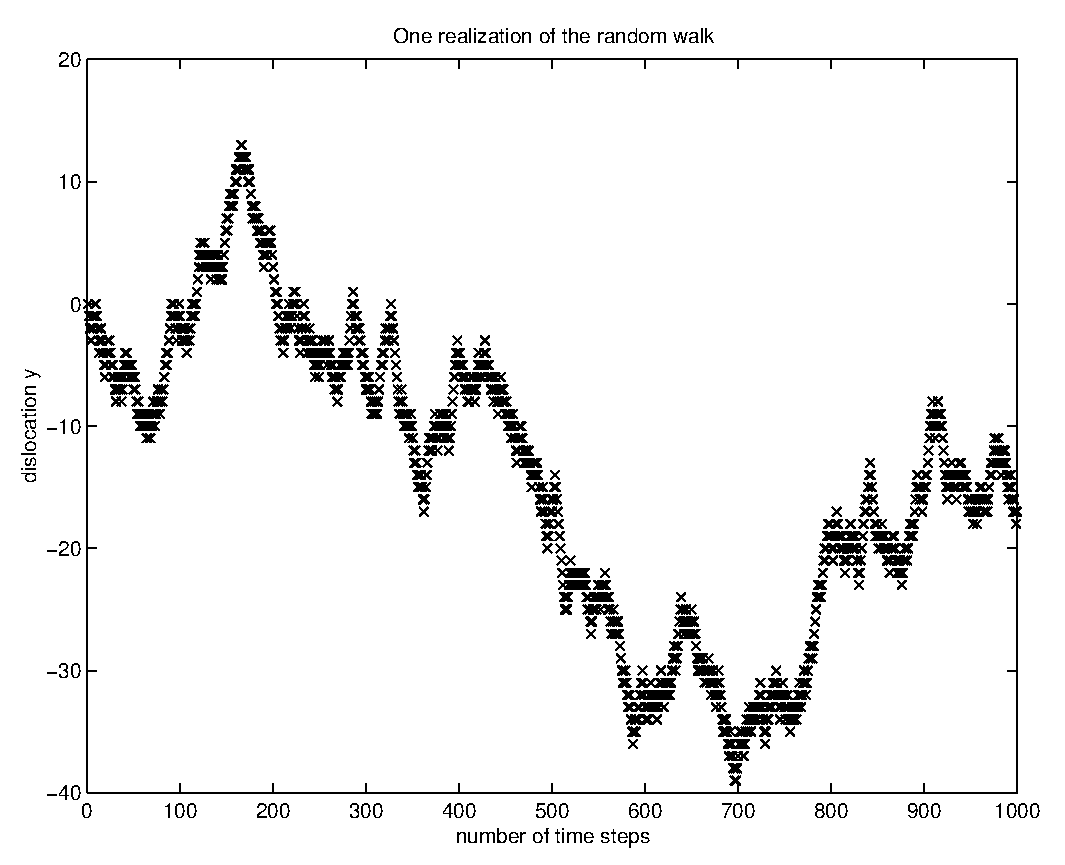
\includegraphics[width=10cm]{./Figures/f_rwdt_2.eps}
\caption{Another realization of a one--dimensional random walk.}
\end{figure}

In order to check the theoretical prediction that the mean square
displacement is proportional to the number of steps we generalize the program
{\sf rwdt} to allow for the generation of more realizations and 
the estimation of the mean value and variance. The new program is called 
{\sf rwdtn} and generates {\sf nreal} realizations of the 
stochastic process.
Its listing can be seen below.

\subsubsection{Listing of the program rwdtn.m}
\inputlisting{./Listings/rwdtn.m}
We run the program for $nstep=100$ and $nreal=1000$. The estimated
mean value of 0.274 and the estimated variance of 103.304 are in quite
good agreement with the theoretical expected vales of 0 nd 100, respectively.
It is interesting to look also at the distribution of the end points of 
the random walk. This can be seen in Fig. (\ref{F_RWDTN}).
\begin{figure}
\label{F_RWDTN}
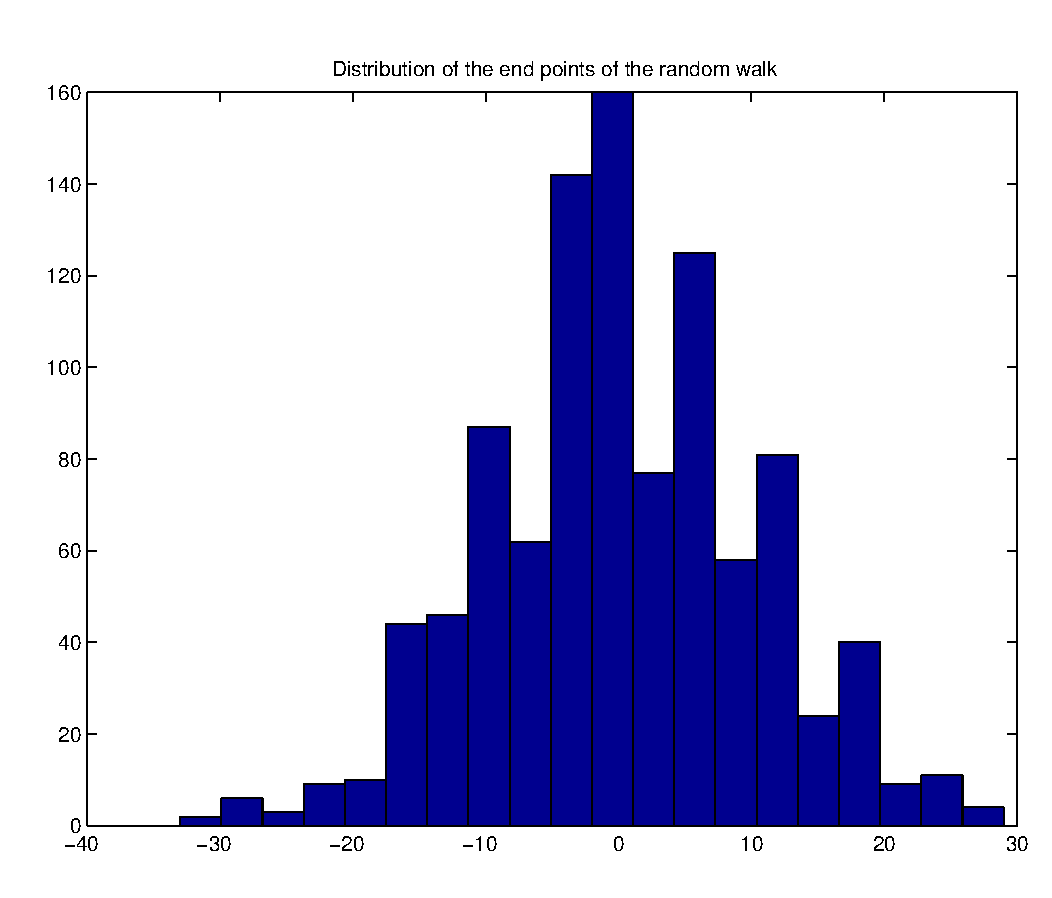
\includegraphics[width=10cm]{./Figures/f_rwdtn.eps}
\caption{The distribution of the end--points of the one--dimensional 
random walk. the program {\sf rwdtn} was run for nstep=100 and 
nreal=1000.}
\end{figure}
\subsection{Generation of Gaussian random numbers}
As a simple demonstration of the central limit theorem we want to 
generate Gaussian distributed random numbers by adding uniformly 
distributed ones.

We know that uniformly distributed random numbers on the interval
$[0,1)$ have $p(x) =1$ for $x\in[0,1)$. Then it is easy to show 
that 
\begin{equation*}
\langle X\rangle = \frac{1}{2}
\end{equation*}
and
\begin{equation*}
{\rm Var}(X) = \int_0^1 x^2 dx - \langle X^2\rangle = \frac{1}{3} 
        -\frac{1}{4} = \frac{1}{12}.
\end{equation*}
Now let us consider the transformed random variable $X'$
\begin{equation*}
X' = (X - \frac{1}{2})\sqrt{12} \sigma
\end{equation*}
which has mean $0$, variance $\sigma^2$, and is uniformly 
distributed on the interval 
$[-\frac{1}{12} \sqrt{12} \sigma, \frac{1}{12} \sqrt{12} \sigma].$
Let us now draw $N$ such random numbers $X'_1,\ldots, X'_N$
and let us construct
the new stochastic variable $Z$
\begin{equation*}
Z= \frac{1}{\sqrt{N}} (X'_1 + \ldots + X'_N).
\end{equation*}
Then the central limit theorem states that the variable $Z$ is a Gaussian
variable with mean $0$ and variance $\sigma^2$.

With the help of the program {\sf cltgen} we want to demonstrate 
that already for $N=12$ we get Gaussian distributed random numbers
in a very good approximation.

\subsubsection{Listing of the program cltgen.m}
\inputlisting{./Listings/cltgen.m}

In Fig. (\ref{F_CLTGEN}) we see the distribution of the Gaussian 
random numbers generated with the help of the program {\sf 
cltgen}. The number of random numbers $Z$ was chosen to be 1000.
\begin{figure}
\label{F_CLTGEN}
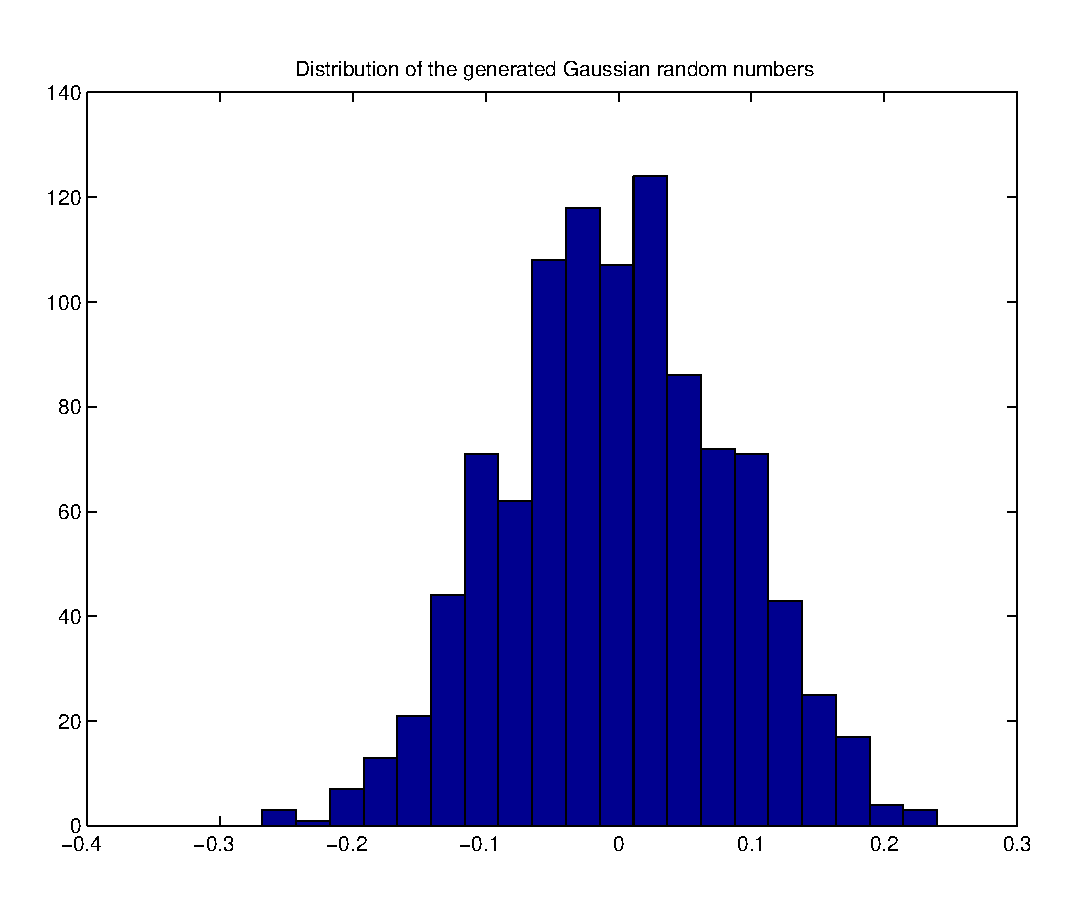
\includegraphics[width=10cm]{./Figures/f_cltgen.eps}
\caption{The distribution of the Gaussian random numbers generate
with the help of the program {\sf cltgen}. The number of random numbers 
drawn was chosen to be $n=1000$.}
\end{figure}

\subsection{Estimation}
{\em Experimental data are random numbers!} An experiment provides
realizations of some random variable $X$. We call an $N$--fold
realization of $X$ a sample of size $N$. It is of fundamental
importance to distinguish between the estimate for the mean and the
variance made on the basis of the sample, which we will denote by $m$
and by $s$, respectively and the corresponding quantities for the
(infinite) underlying population, the ensemble.

Of course, estimates should be unbiased, i.e., for very large samples
the estimate based on the sample size $N$ should converge to the
ensemble averages.

\subsubsection{Mean values}
Let us consider $N$ copies $X_1, \ldots, X_N$  of a random variable
$X$ and let us build the new stochastic variable
\begin{equation*}
Z = \frac{1}{N}(X_1 + \cdots + X_N).
\end{equation*}
$Z$ is the mean value of the $N$ realizations. Assuming that the $X_i$
are uncorrelated we obtain for the cumulants of $Z$
\begin{equation*}
\kappa_n(Z) = \frac{1}{N^n} \sum_{i=1}^N \kappa_n(X_i) =
      N^{-n+1}  \kappa_n(X).
\end{equation*}
In particular we have
\begin{eqnarray*}
\kappa(Z) & = & \langle Z \rangle = \langle X \rangle \\
\kappa_2(Z) & = & {\rm Var}(Z) = \frac{1}{N} \kappa_2(X) = \frac{1}{N}
                  {\rm Var}(X) \\
\kappa_n(Z) & = & O(N^{-2}) \;\;\; {\rm for} \;\; N>2.
\end{eqnarray*}
In other words the mean value of $Z$ is a random variable with a
distribution which has the same mean value as $X$, but with a variance
which is smaller by a factor of $N$. Up to terms of the order
$O(N^{-2})$ the distribution of $Z$ is Gaussian.

\subsubsection{Estimating mean and variance}
Let us consider to have the sample $x_1, \ldots, x_N$. A natural
estimator of the mean value $\mu$ is the sample mean
\begin{equation*}
m= \frac{1}{N} \sum_{i=1}^N x_i.
\end{equation*}
An estimate for the variance could, in analogy, naturally assumed to
be
\begin{equation*}
  \bar{\sigma}^2 = \frac{1}{N} \sum_{i=1}^N (x_i -m)^2.
\end{equation*}
Unfortunately, the above estimator is biased, because we make use of
the already known $m$ instead of the unknown $\mu$. As can easily be
seen
by adding and subtracting $\mu$ in each term in the above equation we
get
\begin {eqnarray*}
 \bar{\sigma}^2 &=& \frac{1}{N} \sum_{i=1}^N [x_i - \mu -(m-\mu)]^2 \\
                & = & \frac{1}{N} \sum_{i=1}^N (x_i - \mu)^2
                              -2(m-\mu)\frac{1}{N} \sum_{i=1}^N (x_i
                                   - \mu)
                           +(m-\mu)^2 \\
               & = & \frac{1}{N} \sum_{i=1}^N (x_i - \mu)^2 - (m-\mu)^2.
\end{eqnarray*}
Now, by taking expectation values averaging over an infinity of samples
of size $N$ we have
\begin{eqnarray*}
E[\bar{\sigma}^2] &= & E\left[\frac{1}{N} \sum_{i=1}^N (x_i - \mu)^2
                                \right]
            - E\left[(m-\mu)^2 \right] \\
       & = & \sigma^2 - \sigma_m^2.
\end{eqnarray*}
If we assume, that there are no correlations we have $\sigma^2_m=
\sigma^2/N$, an unbiased estimate of $\sigma^2$ is
\begin{equation*}
s^2 = \frac{N}{N-1} \bar{\sigma}^2 = \frac{1}{N-1} \sum_{i=1}^N 
      (x_i - m)^2.
\end{equation*}
In computations, if the sample is large, rounding errors can be large
because $(x_i - m)$ is small. In
these cases it is convenient to use the 
"corrected two--pass algorithm" for $s^2$
\begin{equation*}
s^2 = \frac{1}{N-1} \left\{ \sum_{i=1}^N 
      (x_i - m)^2 - \frac{1}{N} \left[\sum_{i=1}^N 
      (x_i - m) \right]^2  \right\}.
\end{equation*}
The function of the additional second term which would be identically
equal to zero if $m$ were exact is to correct the rounding errors of
the first term \cite{PRESS}.

\subsubsection{Confidence levels}
It is important to have also a quantitative characterization of the
goodness of the estimation. To this end we assign to every 
estimation a certain confidence interval, which is to be chosen in 
such a way that the true value lies within this interval at some
predetermined level of confidence. Since we know, by virtue of the
central limit theorem, that the mean value is Gaussian distributed
a criterion for the error can be directly derived from the 
geometric properties of the distribution. Assuming that the
mean value is $m$ and that the standard deviation is
$\sigma_m$ then the probability to find the true value in the
interval $[m-\sigma,n+\sigma]$ is given by the surface 
under a normal probability density
between  $\mu-\sigma_m$ and $\mu + \sigma_m$
\begin{equation*}
{\rm Prob}(\mu \in [m-\sigma,n+\sigma]) =
\int_{m-\sigma}^{m+\sigma} \frac{1}{\sigma \sqrt{2\pi}}
       \exp\left( - \frac{(x-m)^2}{2\sigma^2}\right)
       = 0.683.
\end{equation*}
Thus, in $68.3 \%$ of
samples a value lying within $\pm \sigma_m$  of the population mean
$\mu$ would be found. Conversely, there is $68.3 \%$ probability that
the interval $[m-\sigma_m, m+\sigma_m]$ contains the population mean.

In general we have...

\section{Beyond this chapter}

%%%%%%%%%%%%%%%%%%%%%%%%%%%%%%%%%%%%%%%%%%%%%%%%%%%%%%%%%%%%%%%%%%
\section{Exercises}

\begin{Ex}
\label{Random-Number_Generator_Check}
\textbf{Random-Number Generator Check \cite[]{knuth2:81}} \\
To test the random number generator of Matlab, we calculate the first
10 moments of the distribution generated from \texttt{rand()}.
Compare these with the exact results for a uniform distribution.

Plot a histogram to check for a uniform distribution.

Use the Poker-Test for testing \texttt{rand}: Create many series of 5
random numbers between 1 and 13. Then count the fractions of hands
with two, three and four identical (numbers) cards. Compare the
result with the predictions:
\begin{center}
  \begin{tabular}{lrr}
hand & number of ways& probability\\\hline
all different (no pair) & 1,302,540 & 0.50117739\\
two of a kind & 1,098,240 & 0.42256903\\
three of a kind & 54,912 & 0.021128451\\
four of a kind & 624 & 0.000240096 \\\hline
Total number of possibilities & 2,598,960 & 1
\end{tabular}
\end{center}
For a rigorous check you have to use the chi-squared test for
your results. If you are interested, take a look at the book of D. Knuth.   
\end{Ex}

\begin{Ex}
\label{Galton_Board}
\textbf{Galton Board and Pascal Triangle \cite[]{whitney:90}} \\
Write a program to simulate a Galton Board on the computer.

\begin{center}
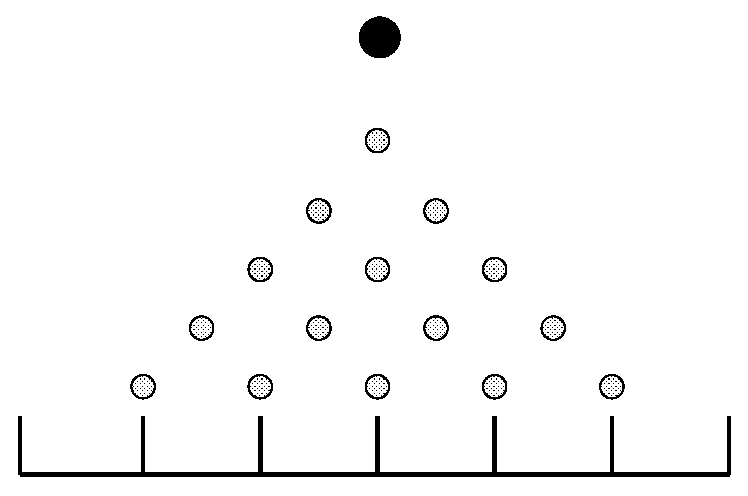
\includegraphics[height=4cm]{Galton_Board.eps}
\end{center}

That is a device where you introduce a ball at the top. The ball
falls down towards the bottom, bouncing off the pins to the right
or left at each level. The only random effect is the bouncing at
the pins at each level. The probability of bouncing to the right or
left is always $0.5$. Therefore it is a simple model for a symmetric
random walk in one dimension.

How can you extract the number of ways to get to one particular
box at the end of the board out of the estimated probabilities above?
What is the connection to the Pascal Triangle?

Change the program to simulate a asymmetric random walk in one
dimension.
\end{Ex}

\begin{Ex}
\label{Standard_Deviation}
\textbf{The Standard Deviation } \\
Compare the four possibilities to calculate the standard deviation
(or the variance):
\begin{enumerate}
\item using the definition: \\
  $$\sigma^2 = \frac{1}{N-1} \sum_{i=1}^N \left( x_i-\overline{x} \right)^2,
    \quad \overline{x} = < x > = \frac{1}{N} \sum_{i=1}^N x_i .$$
\item using the moments: \\
  $$ \sigma^2 = < x^2 > - < x >^2, \quad < x^2 > = \frac{1}{N} 
     \sum_{i=1}^N x_i^2 .$$
\item using the formula (\cite[]{scariano:91}):
  $$ \sigma^2 = \frac{1}{N^2} \sum^N_{\substack{i=1 \\ i<j}} 
      \left( x_i-x_j\right)^2.$$
\item using the corrected two-pass formula \cite[]{recipes}:
  $$ \sigma^2 = \frac{1}{N-1} \left\{\sum_{i=1}^N (x_i-\overline{x})^2
     -\frac{1}{N} \left(\sum_{i=1}^N(x_i-\overline{x}) \right)^2 \right\}.$$
\end{enumerate}
The first and the second method require the computation of the first or
the first and the second moments. The third moment doesn�t require any
precomputed values at all and the last one uses again only the first moment.
The last one corrects for the roundoff errors, encountered when using large
sample sizes. The last one is analytically exact only if $\overline{x}$
would be exact. 

Write a program including all four methods and compare the results.
Find out which method the Matlab function \texttt{std} uses.
Check the calculation with a uniform, a normal and a Cauchy (Lorentz)
distribution. Can you find an example where the two-pass algorithm
is superior to the other ones?

By the way, the variance is not the only value to estimate the
spreading of a sample. Statisticians often use the estimate
$$ \text{adev}\, = \frac{1}{N} \sum_{i=1}^N \left| x_i - \overline{x}\right|$$
as a measure for the distribution width around the mean value.
\end{Ex}

%%%%%%%%%%%%%%%%%%%%%%%%%%%%%%%%%%%%%%%%%%%%%%%%%%%

{\bf Exercise 2} Random variable transformation theorem: (a) Consider 
the linear transorm of X: Y=bX+c. (b) the log--normal 
distribution.
Lit. Gillespie, Am. J. Phys. 51 (1983) 520.
lichkeitstheoretische Grundbegriffe; typische 
Verteilungen (Poisson, Gauss, Binomial); 

%%%%%%%%%%%%%%%%%%%%%%%%%%%%%%%%%%%%%%%%%%%%%%%%%%%%%%%%%%%%%%%%%%


\bibliographystyle{peter}
\bibliography{V_98,simulit}
